%Chapter 8

\renewcommand{\thechapter}{8}

\chapter{Results}\label{sec:results}

%\section{Results}\label{sec:results}

This chapter presents the results of four different experiments: a benchmark suite evaluation of modulo unrolling WU, a strong scaling experiment, a weak scaling experiment, and a block size variation experiment. 

\begin{figure}
\begin{center}
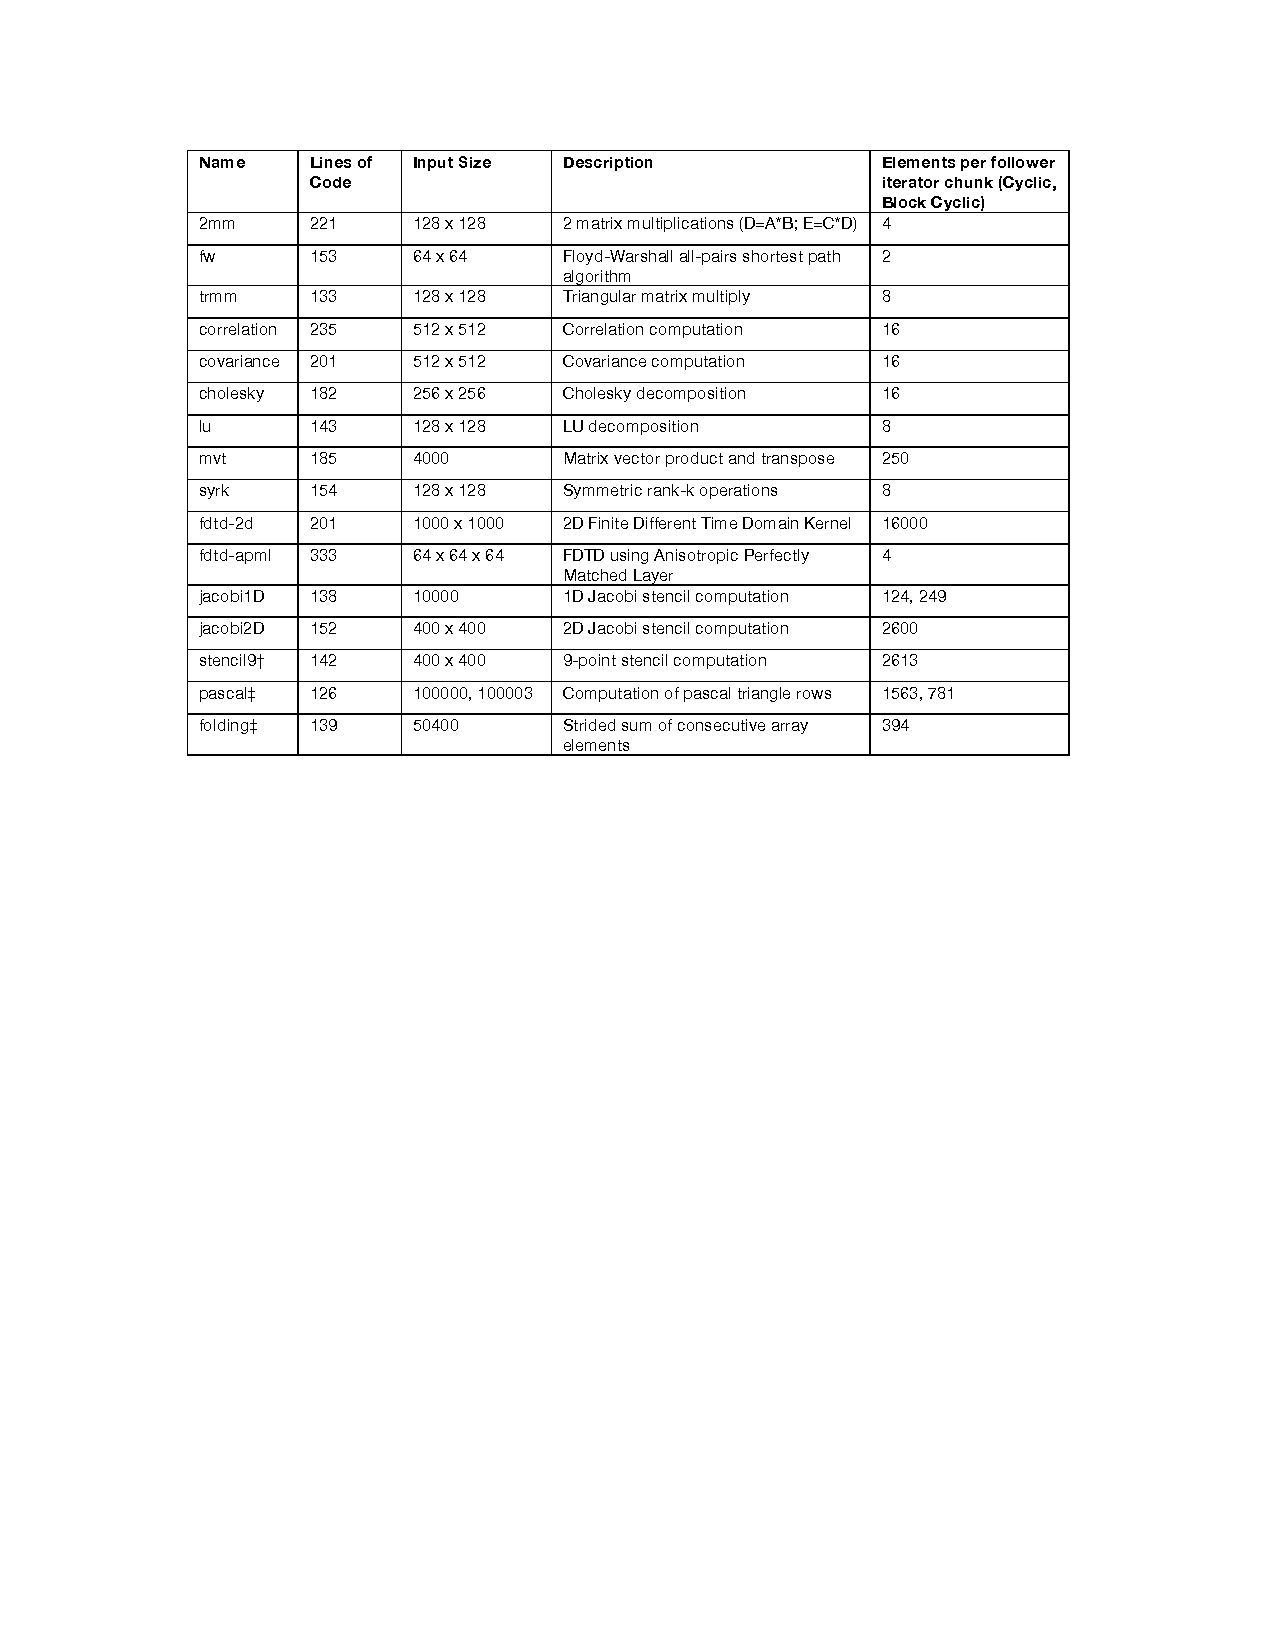
\includegraphics[width=\linewidth]{./Figures/Benchmarks.pdf}
\renewcommand{\baselinestretch}{1}
\small\normalsize
\begin{quote}
\caption[Benchmark suite]{Benchmark suite. Benchmarks with no symbol after their name were taken from the Polybench suite of benchmarks and translated to Chapel. Benchmarks with $\dagger$ are taken from the Chapel Trunk test directory. Benchmarks with $\ddagger$ were developed on our own in order to test specific data access patterns. All benchmarks are tested using the Chapel Cyclic distribution. Only \textit{jacobi1D} and \textit{pascal} are tested using the Chapel Block Cyclic distribution, with block sizes of 4 and 16 respectively. We also measure the maximum number of elements per follower iterator chunk of work for each benchmark to get a sense of how much aggregation is possible.\label{benchmarks}}
\end{quote}
\end{center}
\end{figure}

\section{Benchmark Suite Evaluation}\label{sec:benchmark_suite_evaluation}

To demonstrate the effectiveness of modulo unrolling WU in the Chapel Cyclic and Block Cyclic distributions, we present the results of our benchmark suite evaluation. We have composed a suite of sixteen parallel benchmarks shown in Figure \ref{benchmarks}. Each benchmark is written in Chapel and contains loops with affine array accesses that use zippered iterations, as discussed in Chapter \ref{sec:array_slicing}. This ensures that the leader and follower iterators where modulo unrolling WU is implemented are called. Our suite of benchmarks contains programs with single, double, and triple nested affine loops. Additionally, our benchmark suite contains programs operating on one, two, and three-dimensional distributed arrays. Thirteen of the sixteen benchmarks are taken from the Polybench suite of benchmarks \cite{polybench} and are translated from C to Chapel by hand. The \textit{stencil9} benchmark was taken from the Chapel source trunk directory. The remaining two benchmarks, \textit{pascal} and \textit{folding}, were written by our group. \textit{pascal} is an additional benchmark other than \textit{jacobi1D} that is able to test Block Cyclic with modulo unrolling WU. \textit{folding} is the only benchmark in our suite that has strided affine array accesses. 

To evaluate improvements due to modulo unrolling WU, we ran our benchmarks using the Cyclic and Block Cyclic distributions from the trunk revision 22919 of the Chapel compiler as well as the Cyclic and Block Cyclic distributions that have been modified to perform modulo unrolling WU, as described in Chapter \ref{sec:adaptation_in_chapel}. We measure both runtime and message counts for each benchmark and report the normalized measurements with respect to the existing Chapel Cyclic and Block Cyclic distributions. We also compute the geometric means of all normalized runtimes and message count numbers for both distributions to get a sense of how much improvement, on average, modulo unrolling WU provided for our benchmark suite. 

Data was collected on the ten-locale Golgatha cluster at the Laboratory for Telecommunication Sciences in College Park, Maryland. Each computing node on the cluster is comprised of two 2.93 GHz Intel Xeon X5670 processors, with 24 GB of RAM. The nodes are connected via an InfiniBand network communication link. Benchmarks \textit{fdtd-apml}, \textit{syrk}, \textit{lu}, \textit{mvt}, and \textit{trmm} were run using eight of the ten locales because these programs drew too much power and did not complete execution during data collection when all ten locales were used. The remaining benchmarks were run on ten locales. 

When evaluating modulo unrolling WU used with the Block Cyclic distribution, we only ran two benchmarks (\textit{jacobi1D} and \textit{pascal}) out of our suite of sixteen because of limitations within the original Chapel Block Cyclic distribution. Many of our benchmarks operate on two or three-dimensional arrays and are written using array slicing. Both array slicing of multi-dimensional arrays and array slicing containing strides for one-dimensional arrays are not yet supported in the Chapel compiler's Block Cyclic distribution. Implementing such features remained outside the scope of this work. There was no limitation when evaluating modulo unrolling WU with the Cyclic distribution, and all sixteen benchmarks were tested. Once these missing features are implemented in the Chapel compiler, then our method will apply to all of our benchmarks using the Block Cyclic distribution.

Figure \ref{runtimes} compares the normalized runtime numbers for the Cyclic and Block Cyclic distributions with and without modulo unrolling WU. For ten out of the sixteen benchmarks, we see reductions in runtime when the modulo unrolling WU optimization is applied to the Cyclic distribution. Both benchmarks tested with the Block Cyclic distribution with modulo unrolling WU show reductions in runtime. On average, modulo unrolling WU results in a 36 percent decrease in runtime for Cyclic and a 53 percent decrease in runtime for Block Cyclic. 

\begin{figure}
\begin{center}
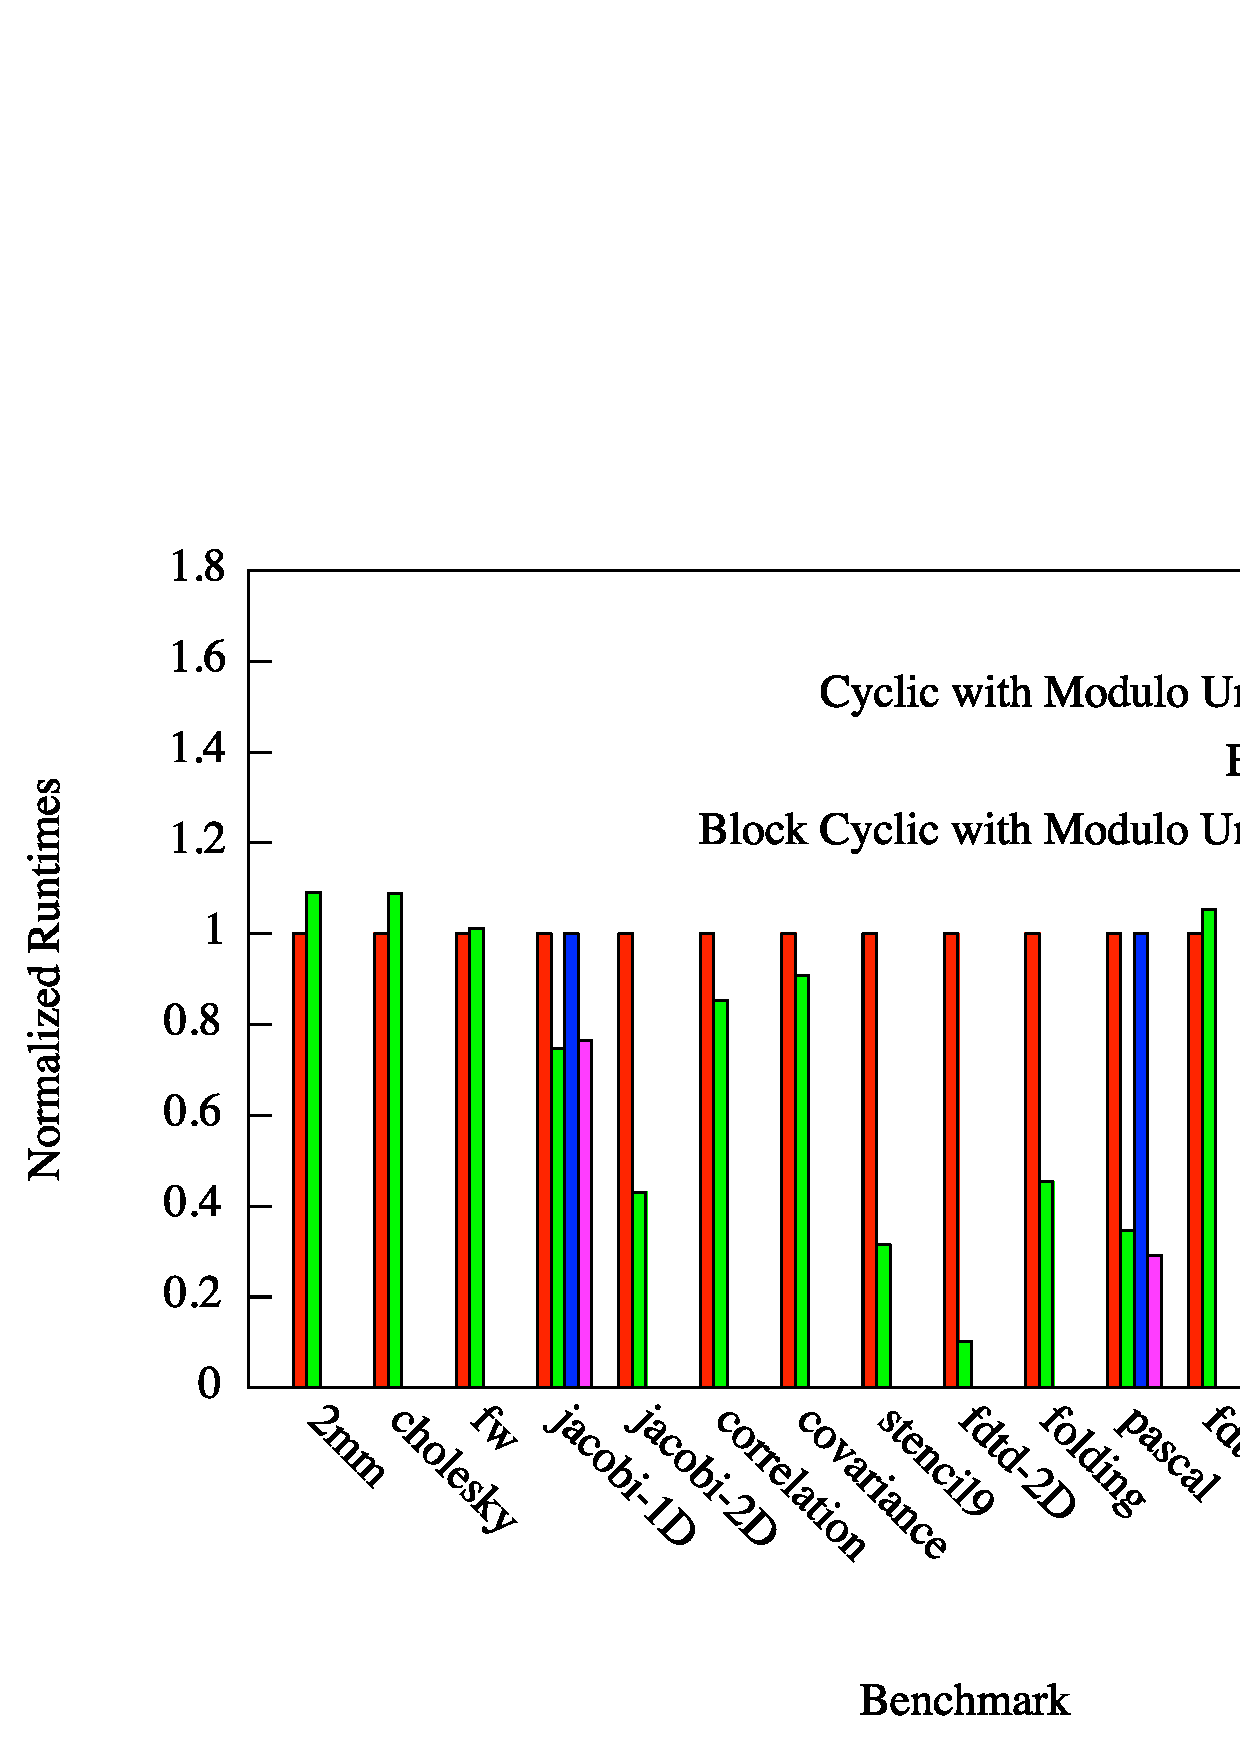
\includegraphics[width=\linewidth]{./Figures/runtimes}
\renewcommand{\baselinestretch}{1}
\small\normalsize
\begin{quote}
\caption[Benchmark suite evaluation: runtime data]{Runtime data collected for our suite of benchmarks. Each measurement is normalized to the benchmark's runtime using the original Chapel Cyclic and Block Cyclic distributions. Measurements below 1 indicate that benchmarks that use modulo unrolling WU with the specified Chapel distribution run faster. The last set of bars reports the geometric means of all sixteen normalized runtimes per distribution. \label{runtimes}}
\end{quote}
\end{center}
\end{figure}

Figure \ref{message_counts} compares the normalized message count numbers for the Cyclic and Block Cyclic distributions with and without modulo unrolling WU. For the Cyclic distribution, nine out of the sixteen benchmarks show reductions in message count 15 percent or greater. Both benchmarks tested with Block Cyclic with modulo unrolling WU show reductions in message count greater than 15 percent. On average, modulo unrolling WU results in a 64 percent decrease in message count for Cyclic and a 72 percent decrease in message count for Block Cyclic. 

\begin{figure}
\begin{center}
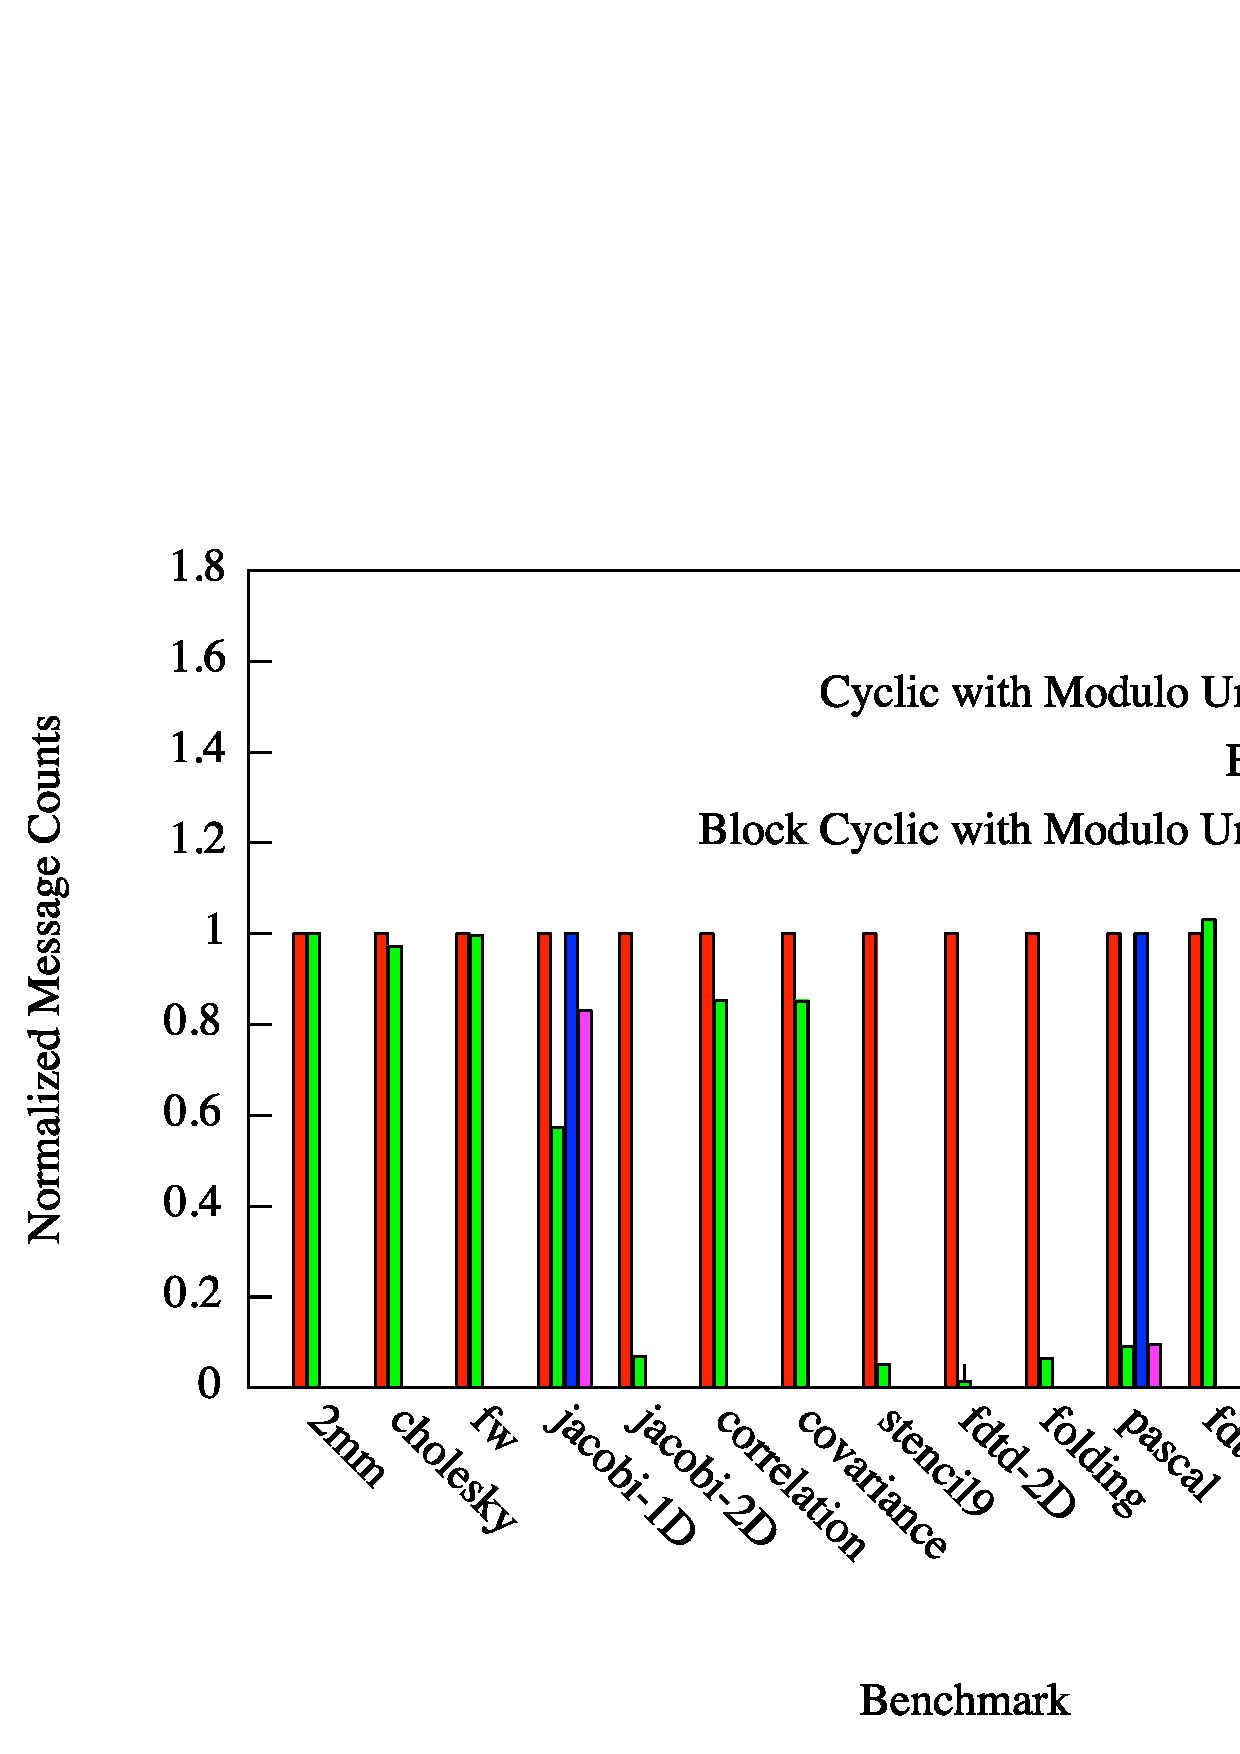
\includegraphics[width=\linewidth]{./Figures/message_counts}
\renewcommand{\baselinestretch}{1}
\small\normalsize
\begin{quote}
\caption[Benchmark suite evaluation: message count data]{Message count data collected for our suite of benchmarks. Each measurement is normalized to the benchmark's message count using the original Chapel Cyclic and Block Cyclic distributions. Measurements below 1 indicate that benchmarks that use modulo unrolling WU with the specified Chapel distribution run using fewer messages. The last set of bars reports the geometric means of all sixteen normalized message counts per distribution.\label{message_counts}}
\end{quote}
\end{center}
\end{figure}

The final column in Figure \ref{benchmarks} shows the maximum number of data elements per follower iterator chunk of work for each benchmark. These numbers, measured experimentally, give us a sense of how many data elements can be aggregated into a single message using modulo unrolling WU. The results of this experiment show that programs with chunks of work each containing more than a few hundred data elements see a significant runtime and message count improvement when using modulo unrolling WU over the original Chapel distributions. 

Some detailed observations on Figures \ref{runtimes} and \ref{message_counts} follow. For six benchmarks that were run using the Cyclic distribution with modulo unrolling WU, runtimes were actually slightly slower and message count numbers either slightly increased or decreased by under 15 percent. Following Figure \ref{benchmarks}, all six of these benchmarks contain follower iterator chunks of work with few data elements. This suggests that, although modulo unrolling WU is applicable to these benchmarks, there are not enough elements to aggregate within each chunk of work to see performance improvments from message aggregation. Unlike individual remote data memory accesses (RDMA) that normally occur during each loop iteration, the strided bulk communication primitives \texttt{chpl\_comm\_gets} and \texttt{chpl\_comm\_puts} that are used in the optimization are not hardware optimized and are slower than RDMA when few data elements are being transferred. However, as the number of data elements per follower iterator chunk increases, we reach a point where the strided bulk communication primitives are faster than individual RDMA transfers. The six benchmarks that used the Cyclic distribution with modulo unrolling WU ran slower because of this overhead. 

Another observation is that the Chapel distributions using modulo unrolling WU use more memory than the originals. The optimization yields elements directly from the local buffer that stores the aggregate message instead of yielding one remote element at a time. This increase in memory overhead is not unique to our scheme -- any method that aggregates messages will necessary use more memory for the aforementioned reason. Although we did not directly measure peak memory usage, this means that each locale on our computer needs at least enough memory to fit the number of elements per follower iterator chunk for each benchmark (see Figure \ref{benchmarks}). This amount of memory is strictly a minimum because it is conceivable for multiple aggregate messages to take up space on a single locale at once, since follower iterator chunks are yielded in parallel. For very large data sets, this behavior could limit the cache performance that we would get when running the original distribution's follower iterator. 

In Chapel, the size of a follower iterator chunk of work used in a parallel zippered loop is determined by many factors including the program's input size, the number of locales that the data is distributed over, the block size parameter (when data is distributed using the Block Cyclic distribution), and most importantly, the number of elements in each object of the zippering. This last factor is closely related to the algorithm of a particular program, and our benchmark suite evaluation has already tested how modulo unrolling WU performs for a variety of algorithms. The remaining sections of Chapter \ref{sec:results} illustrate precisely how changing the parameters of input size, number of locales, and block size affect the performance improvements of modulo unrolling WU.

\begin{figure}
\begin{center}
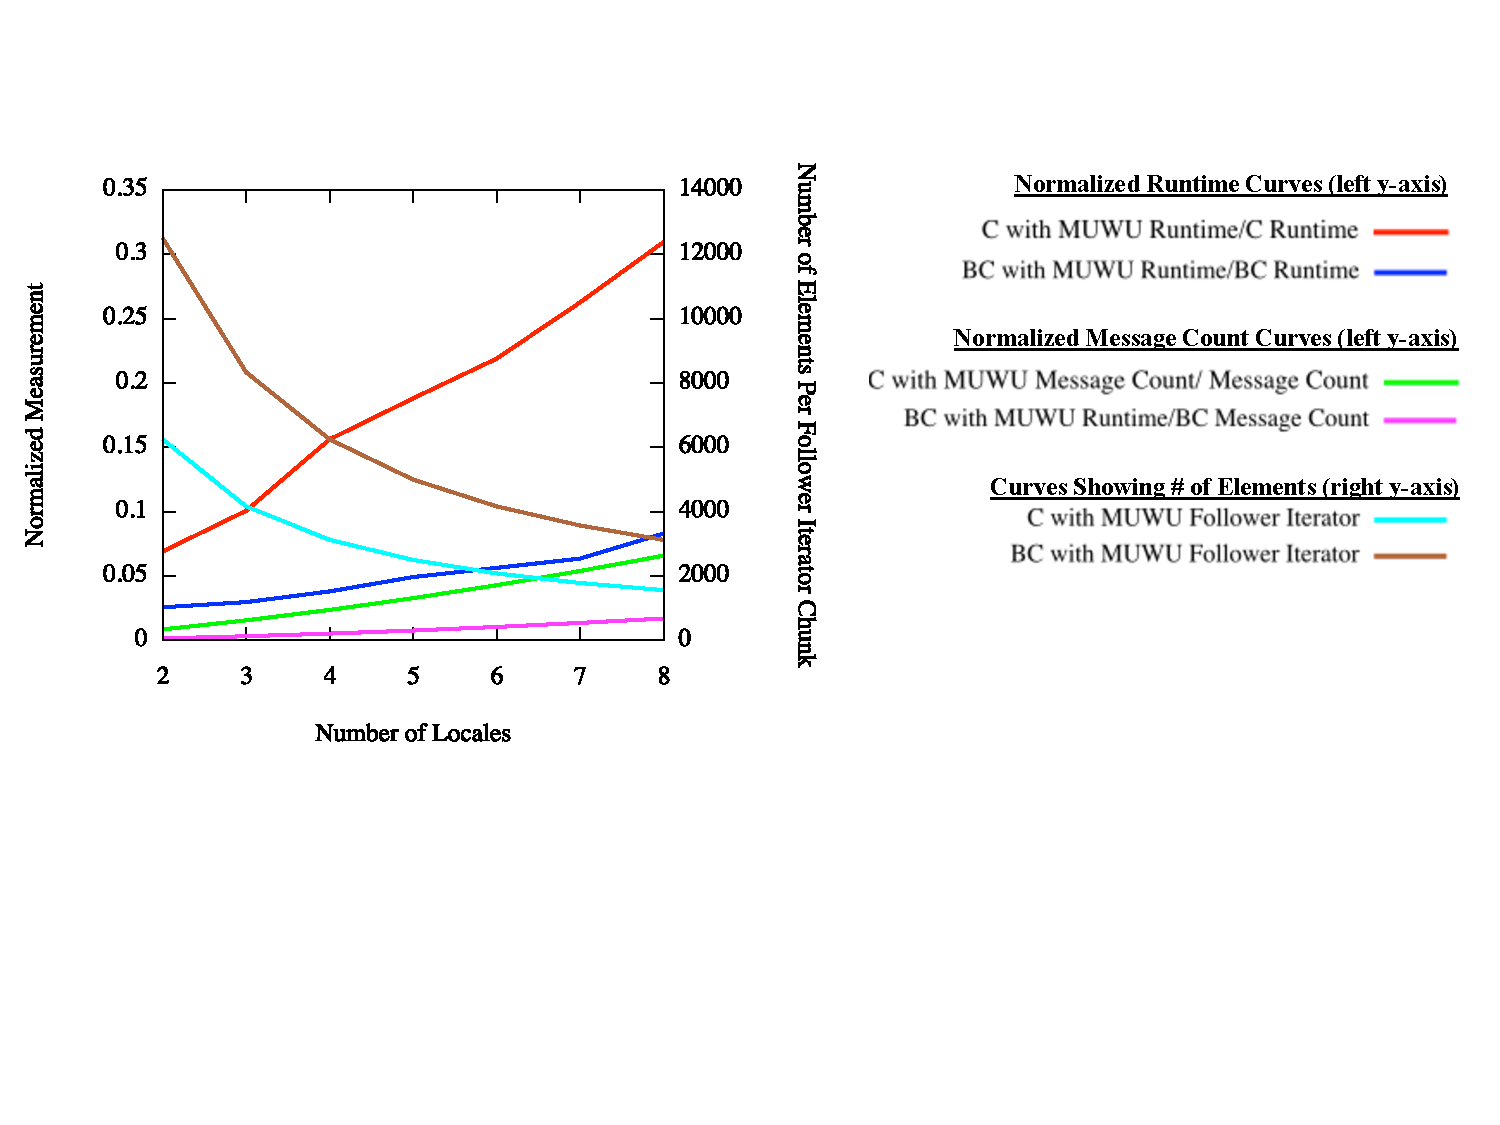
\includegraphics[width=\linewidth]{./Figures/strong_scaling/pascal.pdf}
\renewcommand{\baselinestretch}{1}
\small\normalsize
\begin{quote}
\caption[\textit{pascal} strong scaling results]{\textit{pascal} strong scaling results. For the Block Cyclic results, the block size parameter was 4.\label{pascal_strong_scaling}}
\end{quote}
\end{center}
\end{figure}

\section{Strong Scaling Experiment}\label{sec:strong_scaling}

This experiment tests how strong scaling affects the performance improvements of modulo unrolling WU with the Chapel Cyclic and Block Cyclic distributions. Strong scaling is when a problem of the same size is run using a varying number of locales. Focusing on the following benchmarks -- \textit{pascal}, \textit{folding}, \textit{jacobi2D}, and \textit{fdtd-2d} -- problem sizes stay fixed according to Figure \ref{benchmarks}, but the number of locales varies from two to eight as we measure runtime and message counts relative to the existing Chapel distributions. We also measure the number of elements per follower iterator chunk as a function of the number of locales. 

We choose this subset of benchmarks because they achieved the greatest runtime and communication performance improvements in Chapter \ref{sec:benchmark_suite_evaluation}, while still representing one- and two-dimensional data structures and strided and non-strided data access patterns. In this experiment, \textit{pascal} is the only benchmark used to measure strong scaling for the Chapel Block Cyclic distribution. 

\begin{figure}
\begin{center}
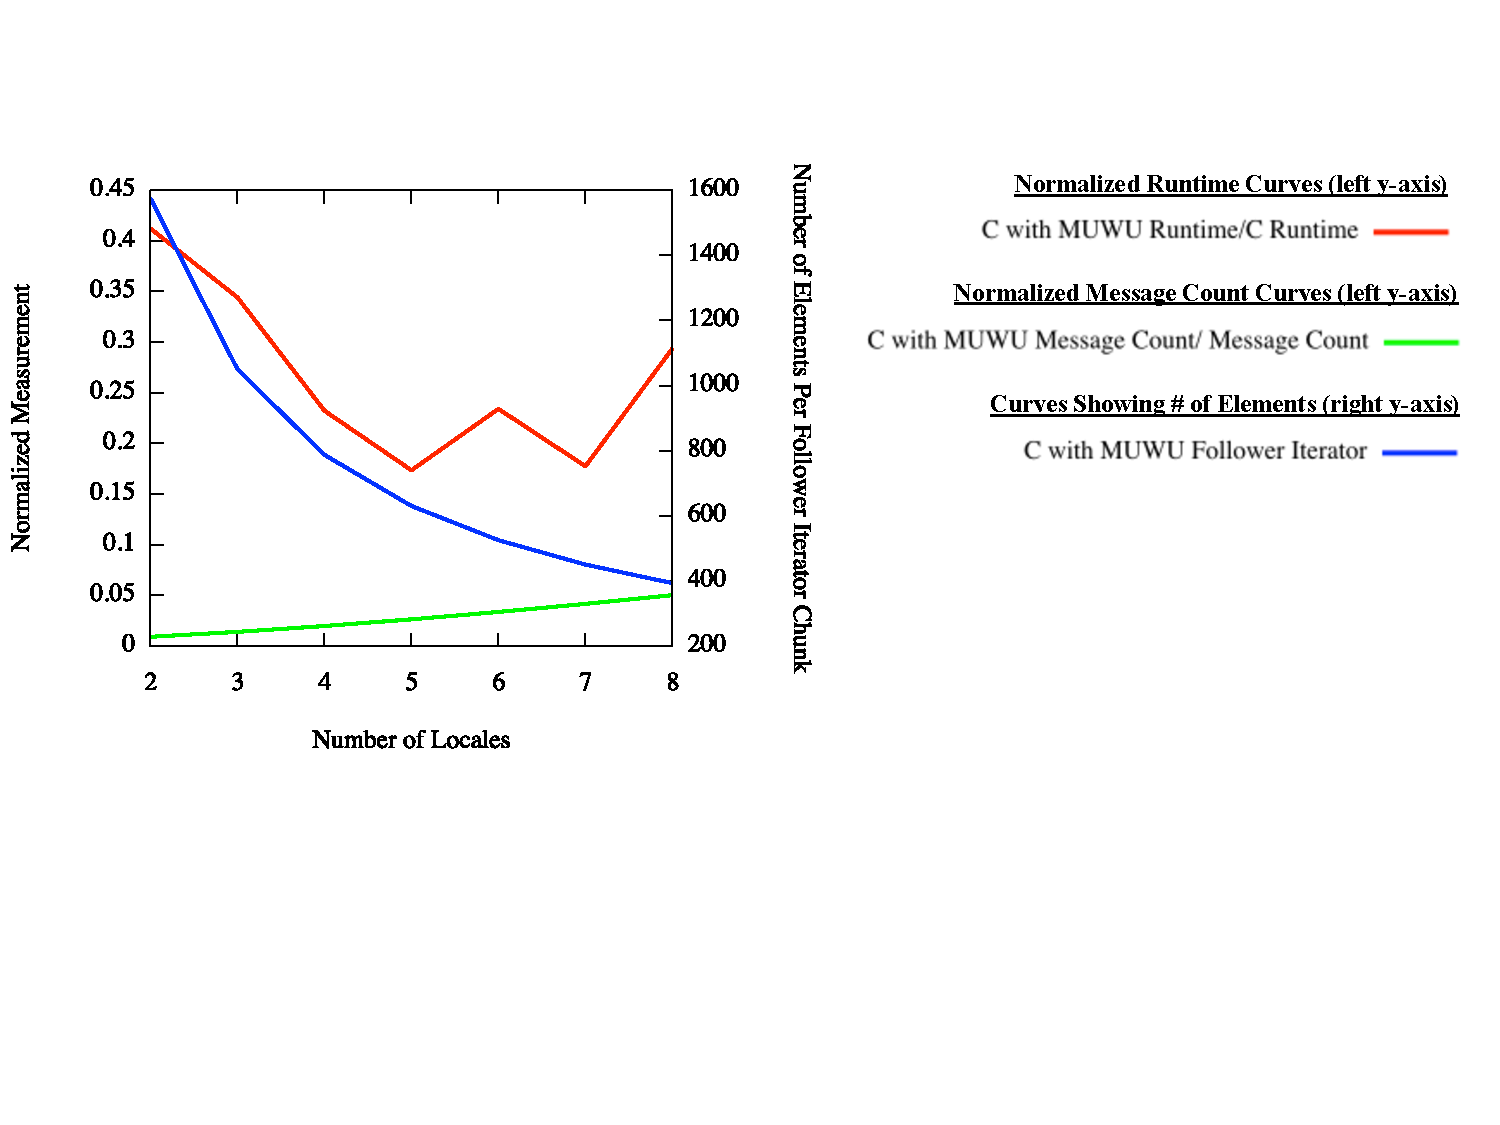
\includegraphics[width=\linewidth]{./Figures/strong_scaling/folding.pdf}
\renewcommand{\baselinestretch}{1}
\small\normalsize
\begin{quote}
\caption[\textit{folding} strong scaling results]{\textit{folding} strong scaling results.\label{folding_strong_scaling}}
\end{quote}
\end{center}
\end{figure}

Figures \ref{pascal_strong_scaling} - \ref{fdtd-2d_strong_scaling} show the strong scaling results for the four benchmarks. We observe the same two trends in each figure. First, the number of elements per follower iterator chunk is inversely proportional to the number of locales that the data is distributed over. This is directly related to the fact that there will be a fewer number of data elements distributed on each locale as more locales are present on the system. Second, as the number of locales increases, both the normalized runtime and message count measurements for modulo unrolling WU increase. This means that the performance improvement gap between modulo unrolling WU and the existing Chapel data distributions gets smaller as the number of locales increases. We attribute the decrease in performance improvement of modulo unrolling WU to be caused by fewer elements available to be aggregated as the number of locales increases.  

\begin{figure}
\begin{center}
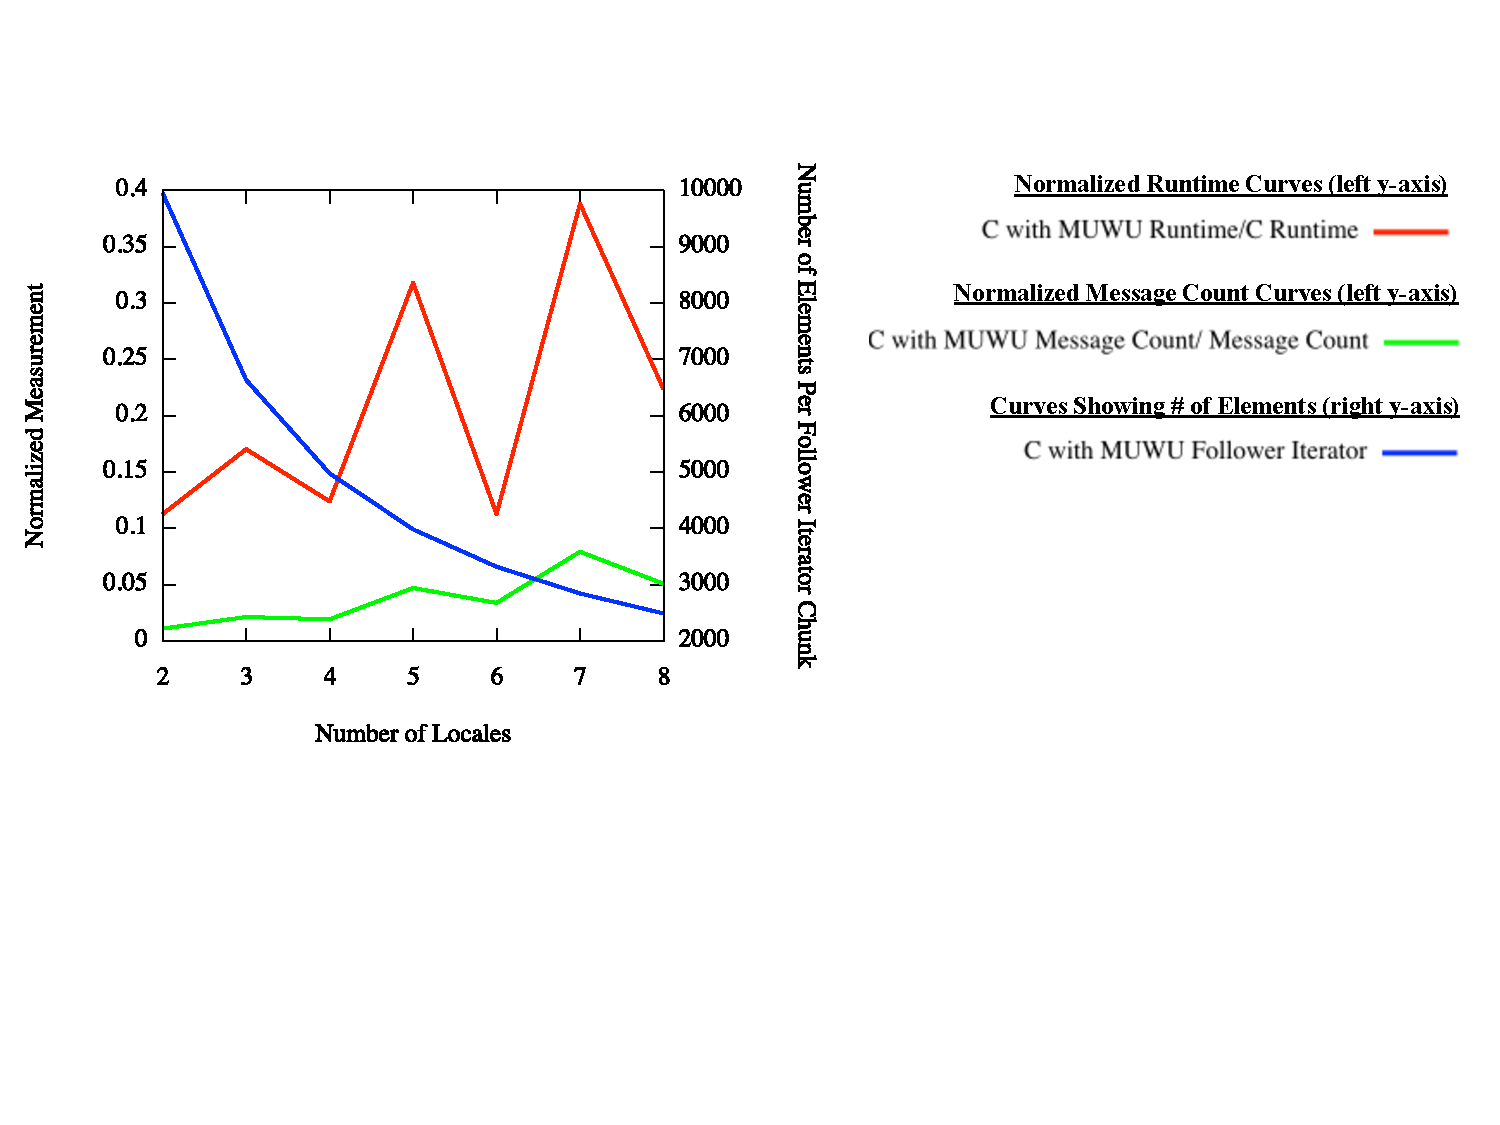
\includegraphics[width=\linewidth]{./Figures/strong_scaling/jacobi-2d.pdf}
\renewcommand{\baselinestretch}{1}
\small\normalsize
\begin{quote}
\caption[\textit{jacobi2D} strong scaling results]{\textit{jacobi2D} strong scaling results.\label{jacobi-2d_strong_scaling}}
\end{quote}
\end{center}
\end{figure}

In Figures \ref{jacobi-2d_strong_scaling} and \ref{fdtd-2d_strong_scaling}, which correspond to the strong scaling results for the \textit{jacobi2D} and \textit{fdtd-2d} benchmarks respectively, we observe spikes in the normalized runtime and message count measurements for some numbers of locales, even though the overall trend still increases when more locales are added. Both the \textit{jacobi2D} and \textit{fdtd-2d} benchmarks happen to operate on two-dimensional arrays and contain nearest neighbor computation. When distributing data cyclically in Chapel, by default the pattern that the Cyclic distribution tries to assign elements to locales is as ``square" or ``rectangular" as possible. For example, in Figure \ref{cyc_dist}, the two-dimensional array is distributed over four locales using a 2x2 pattern. However, with four locales, this same array could have been distributed using a 4x1 or 1x4 linear pattern. It turns out that for benchmarks similar to \textit{jacobiD} and \textit{fdtd-2d}, using a "rectangular" pattern will result in more remote data accesses per loop iteration than a linear pattern, leading to a higher improvement when message aggregation is applied. The spikes we see in Figures \ref{jacobi-2d_strong_scaling} and \ref{fdtd-2d_strong_scaling} occur when we distribute the data over a prime number of locales. In this case, the only pattern to use to distribute a two-dimensional array over a prime number $n$ locales is a linear pattern of $n$x1 or 1x$n$. Note that it is possible to specify such patterns explicitly in Chapel for composite number of locales. 

\begin{figure}
\begin{center}
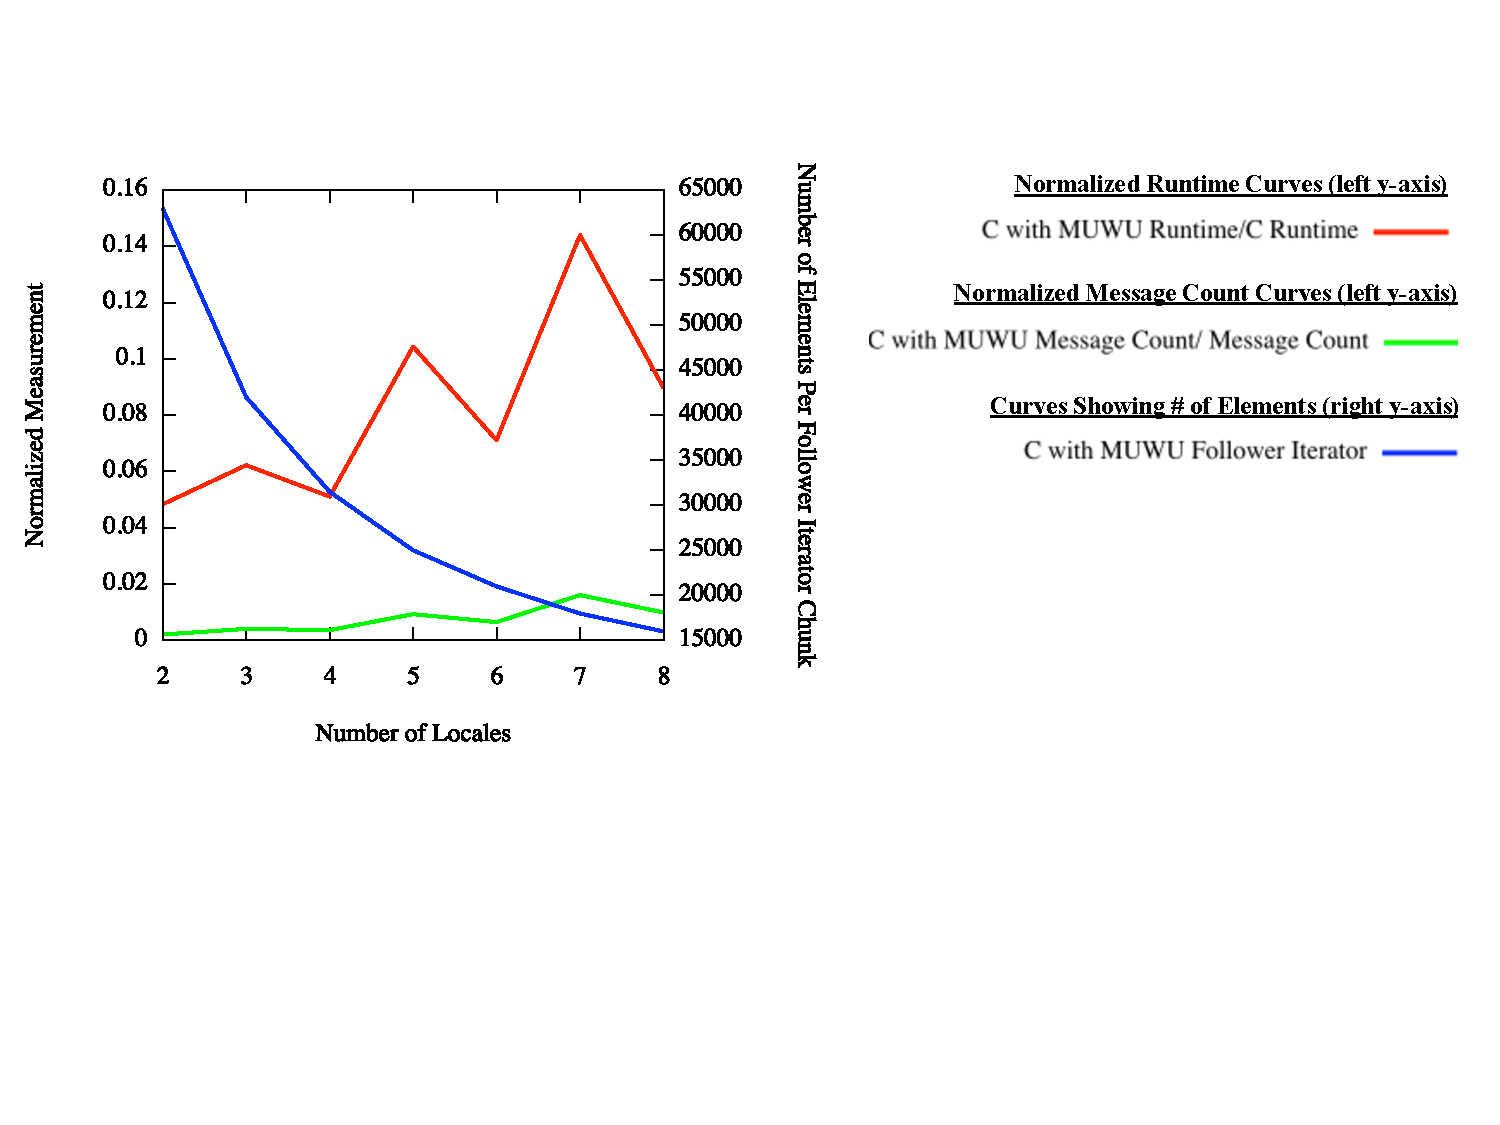
\includegraphics[width=\linewidth]{./Figures/strong_scaling/fdtd2d.pdf}
\renewcommand{\baselinestretch}{1}
\small\normalsize
\begin{quote}
\caption[\textit{fdtd-2d} strong scaling results]{\textit{fdtd-2d} strong scaling results.\label{fdtd-2d_strong_scaling}}
\end{quote}
\end{center}
\end{figure}

\section{Weak Scaling Experiment}\label{sec:input_variation}

\begin{figure}
\begin{center}
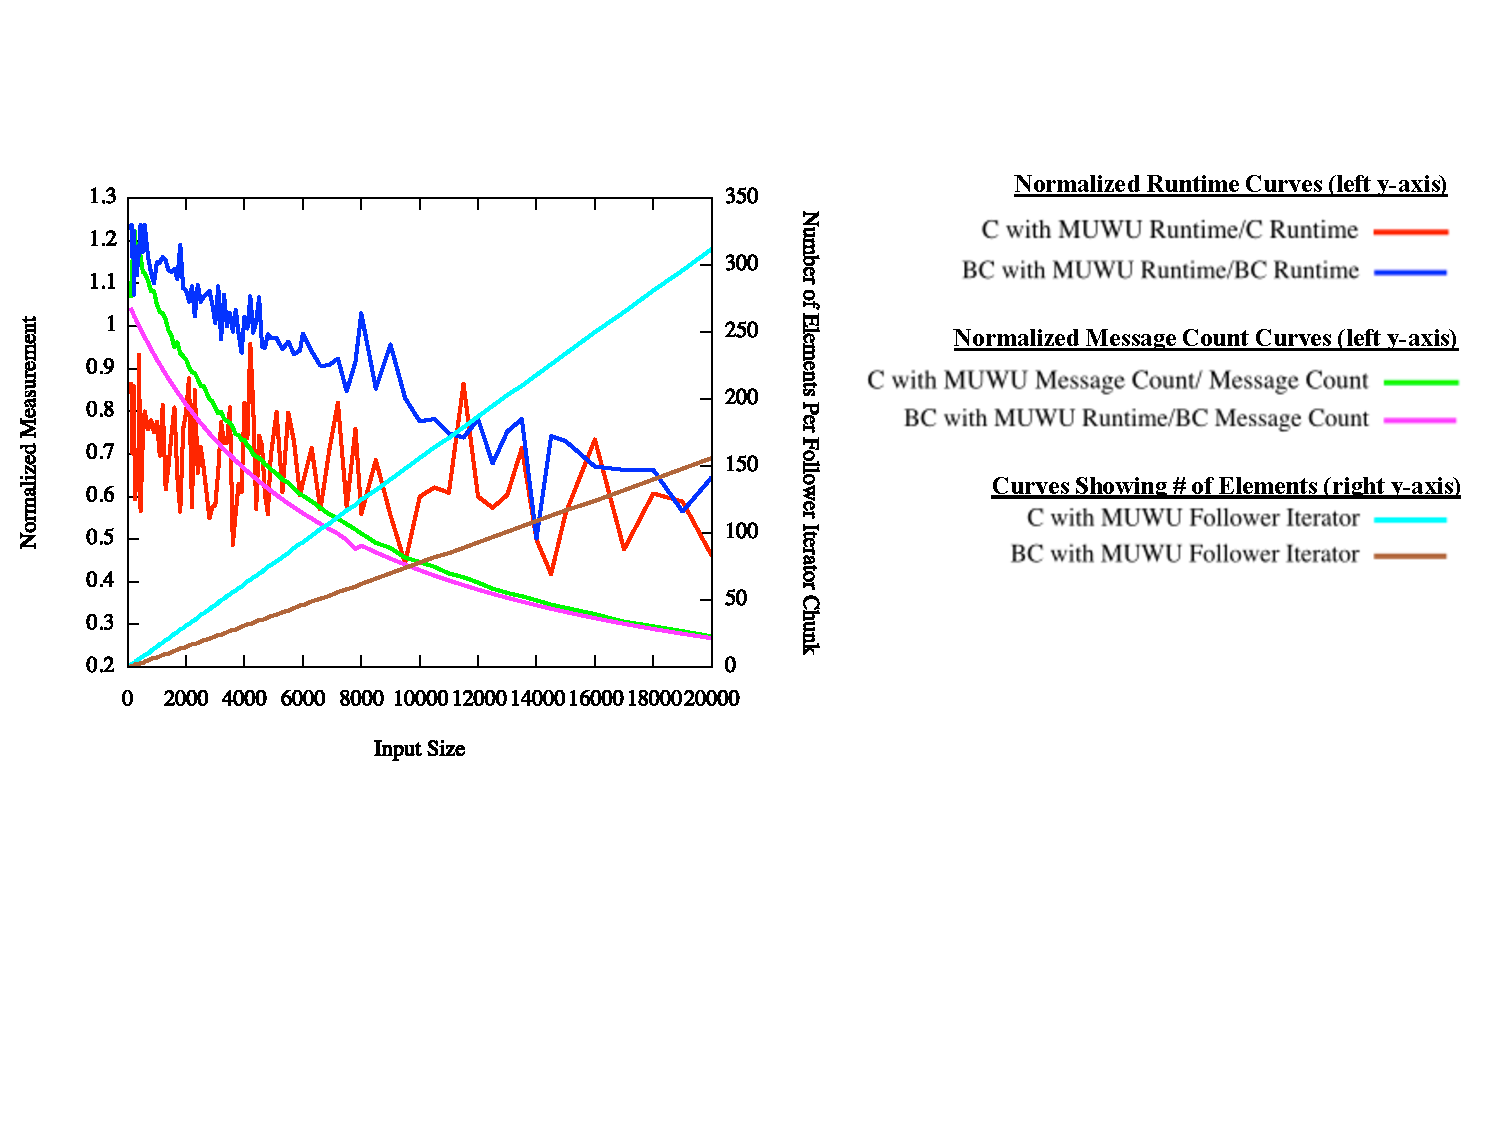
\includegraphics[width=\linewidth]{./Figures/input_variation_exp/pascal.pdf}
\renewcommand{\baselinestretch}{1}
\small\normalsize
\begin{quote}
\caption[\textit{pascal} weak scaling results]{\textit{pascal} weak scaling results. For the Block Cyclic results, the block size parameter is 16.\label{pascal_weak_scaling}}
\end{quote}
\end{center}
\end{figure}

This experiment tests how weak scaling affects the relative performance of modulo unrolling WU with the Chapel Cyclic and Block Cyclic distributions. Weak scaling is when we run programs on a constant number of locales but vary the input size as we measure the performance.The same benchmarks used to measure strong scaling in Chapter \ref{sec:strong_scaling} are also used here to measure weak scaling. Varying the input size of our benchmarks and keeping the number of locales constant at eight, we measure the runtimes and message counts normalized to the existing Chapel distributions. Once again, \textit{pascal} is the only benchmark used to measure weak scaling for the Chapel Block Cyclic distribution. 

Figures \ref{pascal_weak_scaling} - \ref{fdtd-2d_weak_scaling} show the weak scaling results for the four benchmarks. We observe some similar trends throughout each benchmark. First, normalized message counts are inversely proportional to the input size of the benchmark, and this is evident for both the Cyclic and Block Cyclic distributions. As input size increases, we observe that the absolute message count measurements continue to increase when modulo unrolling WU is not used because each remote data access requires its own message. When modulo unrolling WU is used, absolute message count measurements increase until a maximum and then stop increasing, due to aggregation, even when input size continues to increase. Normalized runtime also appears to be inversely proportional to input size, but a given benchmark's normalized runtime for a particular input size is not predictable. Finally, as input size increases, so does the number of elements per follower iterator chunk for both the Cyclic and Block Cyclic distributions, implying that larger input sizes do indeed create a greater opportunity for message aggregation. The number of elements per follower iterator chunk increases linearly for the \textit{pascal} and \textit{folding} benchmarks and quadratically for the \textit{jacobi2D} and \textit{fdtd-2d} benchmarks.

\begin{figure}
\begin{center}
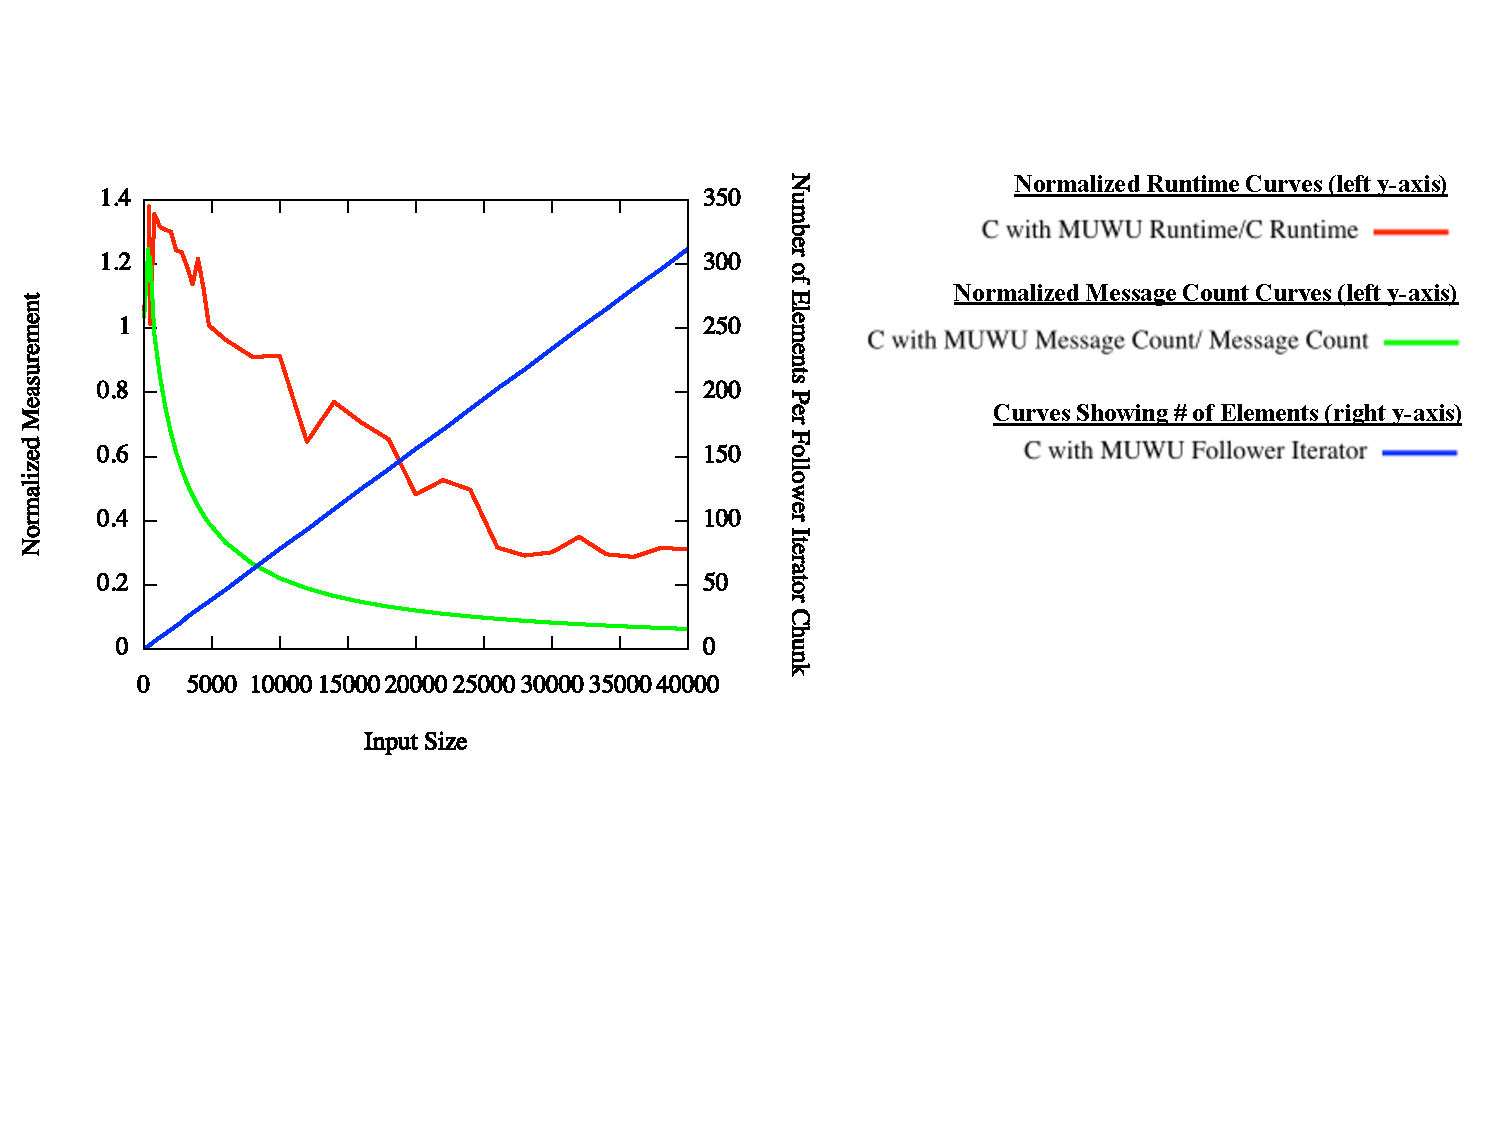
\includegraphics[width=\linewidth]{./Figures/input_variation_exp/folding.pdf}
\renewcommand{\baselinestretch}{1}
\small\normalsize
\begin{quote}
\caption[\textit{folding} weak scaling results]{\textit{folding} weak scaling results.\label{folding_weak_scaling}}
\end{quote}
\end{center}
\end{figure}

\begin{figure}
\begin{center}
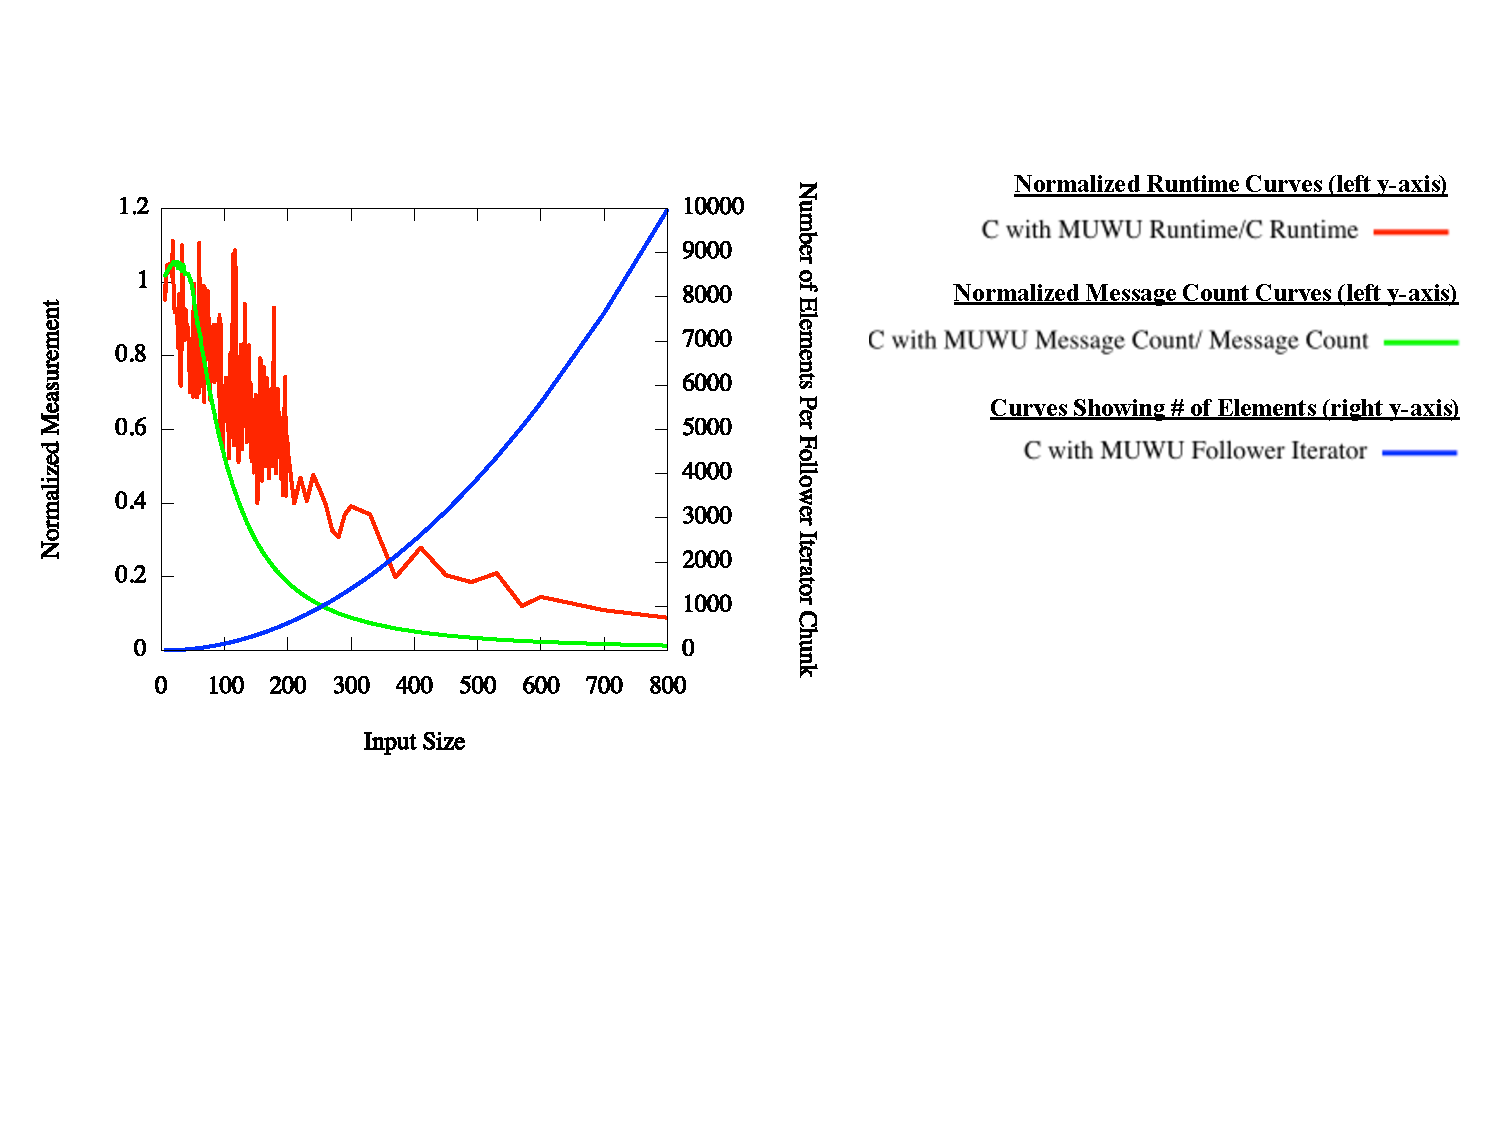
\includegraphics[width=\linewidth]{./Figures/input_variation_exp/jacobi-2d.pdf}
\caption{\textit{jacobi2D} weak scaling results.\label{jacobi-2d_weak_scaling}}
\end{center}
\end{figure}

\begin{figure}
\begin{center}
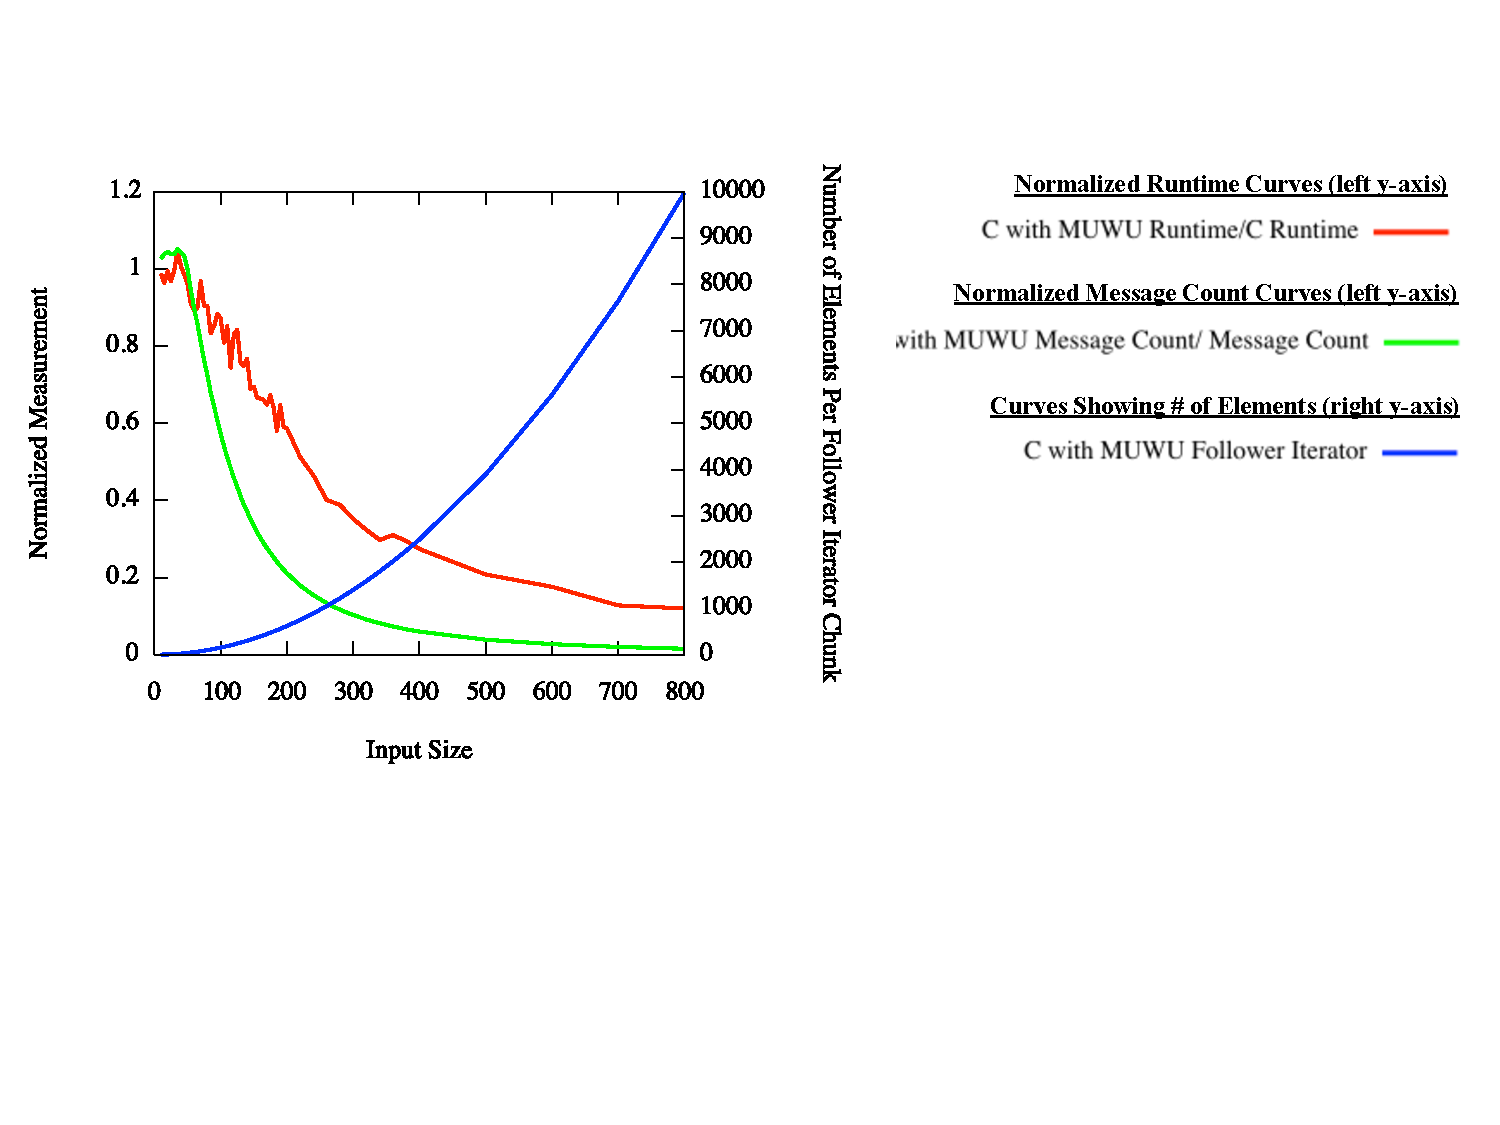
\includegraphics[width=\linewidth]{./Figures/input_variation_exp/fdtd2d.pdf}
\renewcommand{\baselinestretch}{1}
\small\normalsize
\begin{quote}
\caption[\textit{fdtd-2d} weak scaling results]{\textit{fdtd-2d} weak scaling results.\label{fdtd-2d_weak_scaling}}
\end{quote}
\end{center}
\end{figure}

\section{Block Size Variation Experiment}\label{sec:blocksize_variation}

\begin{figure}
\begin{center}
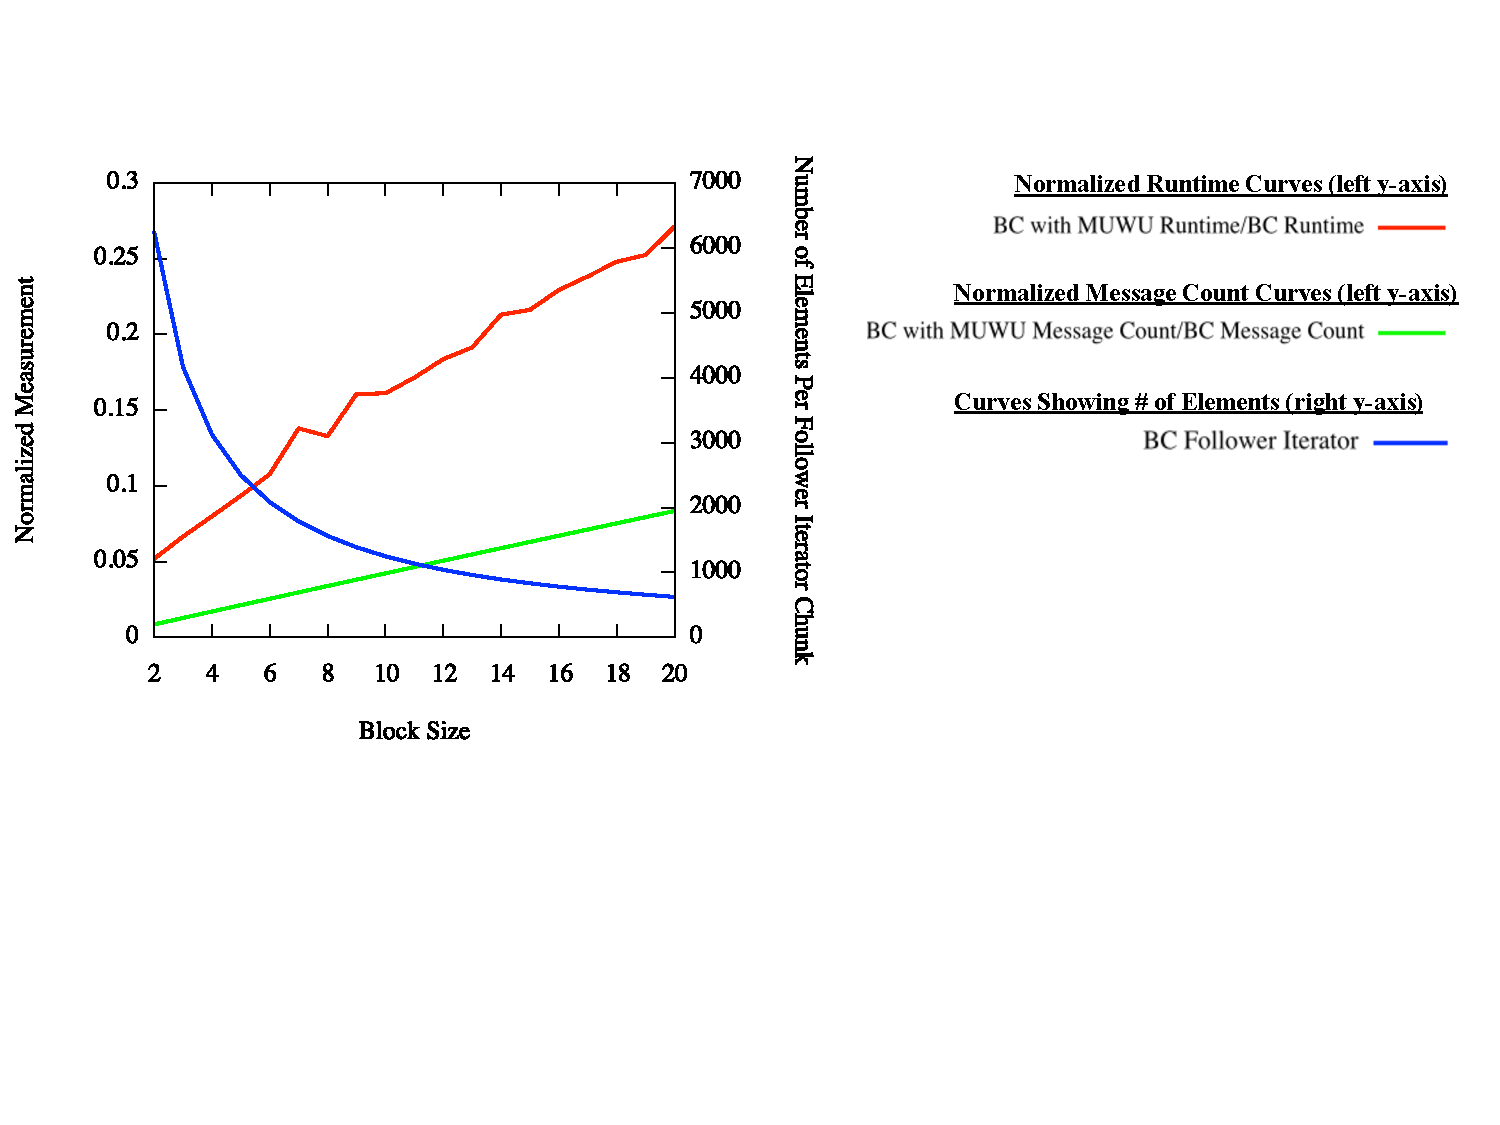
\includegraphics[width=\linewidth]{./Figures/blocksize_variation_exp/pascal.pdf}
\renewcommand{\baselinestretch}{1}
\small\normalsize
\begin{quote}
\caption[\textit{folding} block size variation results]{\textit{folding} block size variation results.\label{folding_blocksize_scaling}}
\end{quote}
\end{center}
\end{figure}

In this experiment, we focus on the two benchmarks \textit{pascal} and \textit{jacobi1D}, where the Chapel Block Cyclic distribution can be used to distribute data, in order to assess the effect of block size on the runtime and communication performance of modulo unrolling WU. We vary the block size parameter (keeping input sizes constant according to Figure \ref{benchmarks} and the number of locales constant at eight) as we measure runtimes and message counts relative to the existing Chapel distributions. 

Figures \ref{folding_blocksize_scaling} and \ref{jacobi1D_blocksize_scaling} show the results of the block size variation experiment for the \textit{folding} and \textit{jacobi1D} benchmarks, respectively. For both benchmarks, we observe that as block size increases, the relative performance improvement of modulo unrolling WU decreases. This is because increasing block size generally decreases the number of elements per follower iterator chunk, which lowers the amount of aggregation possible. 

\begin{figure}
\begin{center}
\renewcommand{\baselinestretch}{1}
\small\normalsize
\begin{quote}
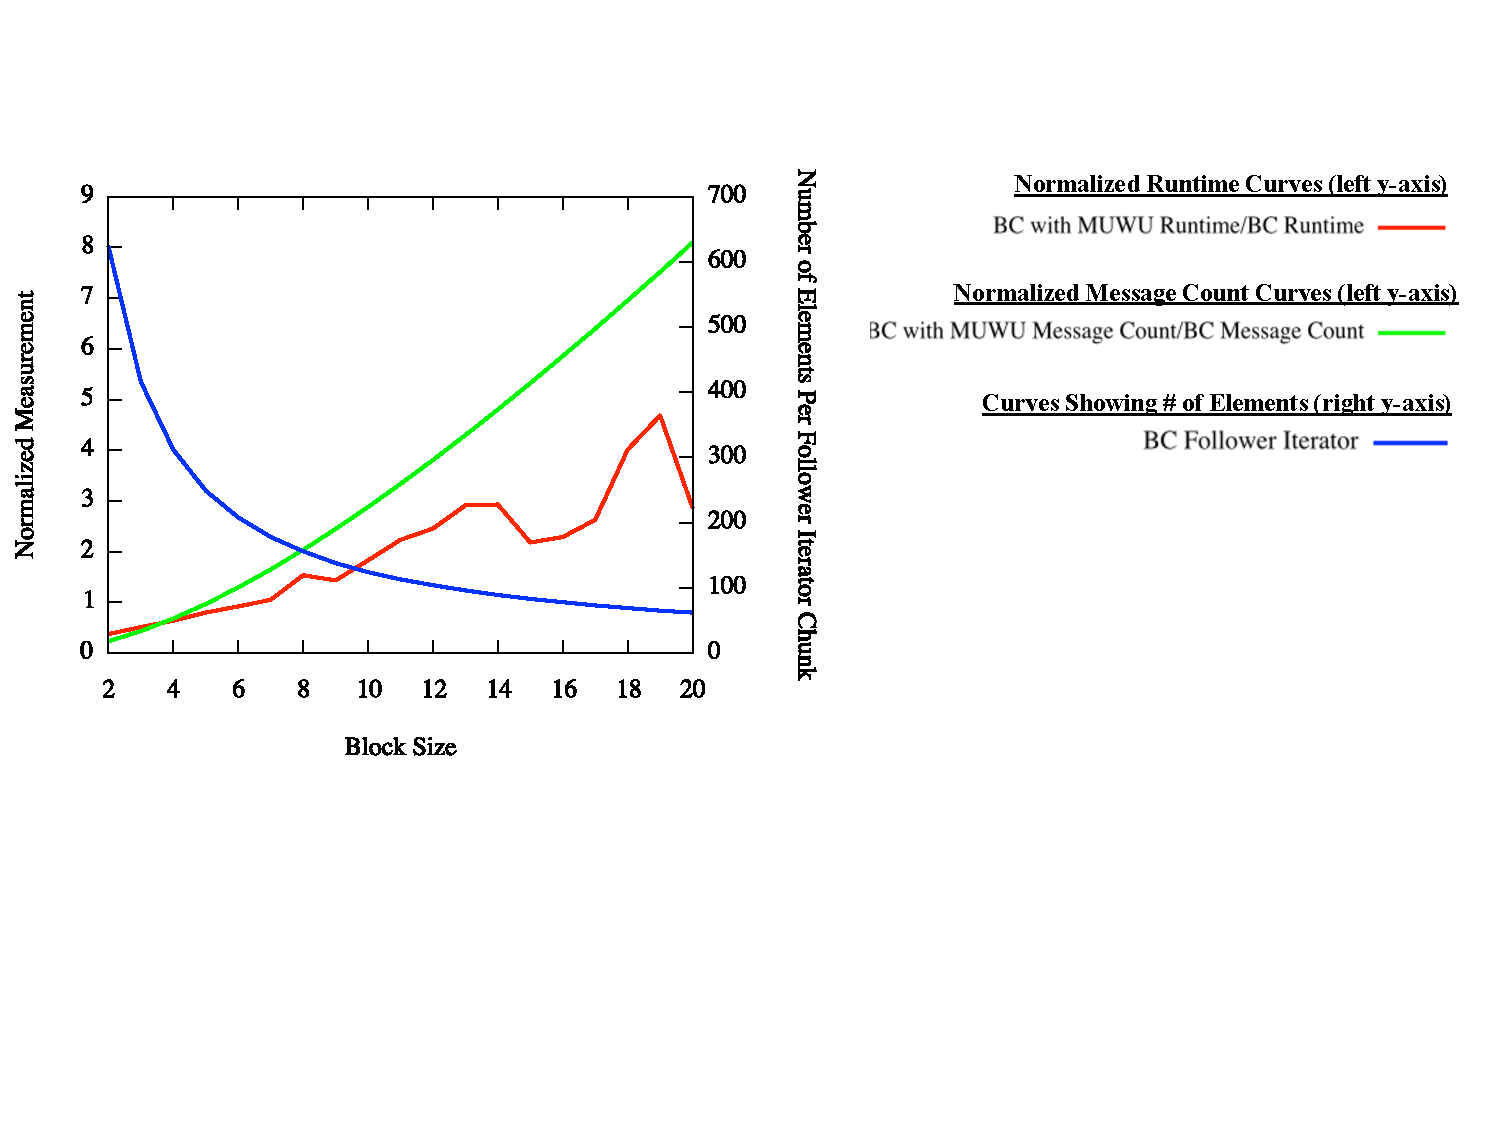
\includegraphics[width=\linewidth]{./Figures/blocksize_variation_exp/jacobi-1d.pdf}
\caption[\textit{jacobi1D} block size variation results]{\textit{jacobi1D} block size variation results.\label{jacobi1D_blocksize_scaling}}
\end{quote}
\end{center}
\end{figure}